% !TeX root = ../../main.tex
\chapter{Umsetzung}\label{sec:implementation}
Im folgenden wird der Aufbau des Projektes sowie verwendete Bibliotheken erläutert.
Zusätzlich wird auf die Implementierung der einzelnen Schritte der SfM Pipeline eingegangen.
Die einzelnen Schritte der Pipline sind teilweise in unterschiedlichen Klassen implementiert.
Die \autoref{fig:pipeline-classes} gibt einen Überblick über diese sowie deren Beziehungen zueinander.

\begin{figure}
    \centering
    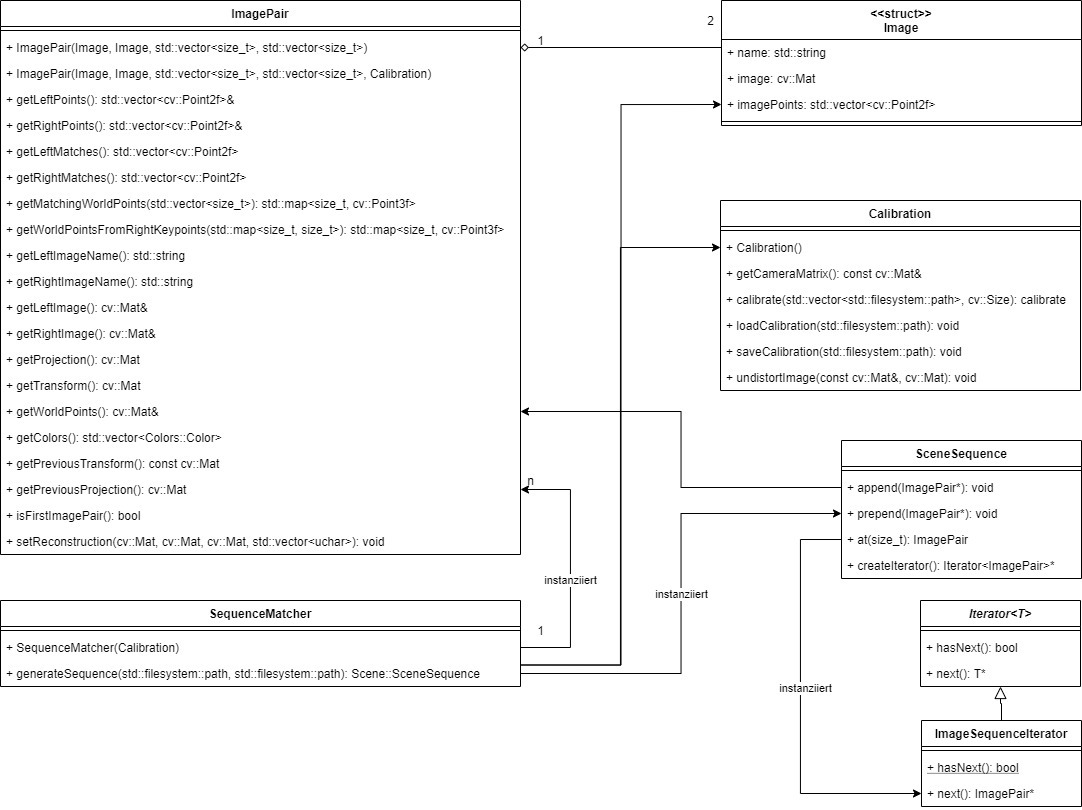
\includegraphics[width=\textwidth]{src/img/classes.jpg}
    \caption{Klassendiagramm alle Klassen welche Pipeline Funktionen implementieren}
    \label{fig:pipeline-classes}
\end{figure}

\section{Projektstruktur}\ohead{Sebastian Schmitt}
Die Applikation wird in C++ entwickelt.
Auch wenn Performance kein Ziel ist, wurde C++ gewählt um eine höhere Performance zu erreichen.
Einzige Abhängigkeit ist die offene Bibliothek OpenCV, siehe dazu \ref{sec:opencv}.
Zur Buildsteuerung wird das quelloffene Tool CMake\footnote{https://cmake.org/} verwendet.

Das Projekt ist folgendermaßen strukturiert:

\dirtree{%
.1 yapgt.
.2 include \ldots{} \begin{minipage}[t]{12cm}
Header-Dateien
\end{minipage}.
.2 resources \ldots{} \begin{minipage}[t]{12cm}
Bilder zum Testen von Kalibrierung und Feature-Matching
\end{minipage}.
.2 src \ldots{} \begin{minipage}[t]{12cm}
Implementierung
\end{minipage}.
.2 CMakeLists.txt \ldots{} \begin{minipage}[t]{12cm}
CMake Konfiguration
\end{minipage}.
}


\section{OpenCV}\label{sec:opencv}
Es wird OpenCV in der Version 4.2.0 mit dem Modul OpenCV Contrib verwendet.
OpenCV Contrib beinhaltet OpenCV Module, welche jedoch nicht stabil genug sind um Teil der offiziellen OpenCV Distribution zu sein \cite[README.md]{opencv_2013}.
OpenCV wurde mit folgenden Optionen kompiliert:
\begin{itemize}
	\item OPENCV\_EXTRA\_MODULES\_PATH um den Pfad zu OpenCV Contrib festzulegen
	\item OPENCV\_ENABLE\_NONFREE um auch nicht freie Algorithmen zu kompilieren
\end{itemize}
Auch wenn es Anforderung ist nur freie Bibliotheken zu verwenden, ist der Flag OPENCV\_ENABLE\_NON\_FREE notwendig.
Der in dieser Arbeit verwendete Algorithmus Scale-Invariant Feature Transform (SIFT) war bis 06. März 2020 von der University of British Columbia patentiert\footnote{siehe dazu https://patents.google.com/patent/US6711293} und ist daher in der verwendeten OpenCV Version nur mit OPENCV\_ENABLE\_NON\_FREE nutzbar.
SIFT ist Teil des Moduls Features2D extra (xfeatures2d) welches Teil von OpenCV Contrib ist und sowohl experimentelle als auch nicht freie Algorithmen beinhaltet.

Um die Applikation auch nutzen zu können ohne vorab OpenCV zu installieren oder zu kompilieren wurde CMake angewiesen, OpenCV statisch zu linken (siehe \autoref{lst:cmake_opencv_static}, Zeilen 1-4).
Zusätzlich kopiert CMake alle gelinkten Bibliotheken, auch wenn diesen nicht referenziert werden, in den Ausgabeordner, damit diese nicht von Hand kopiert werden müssen (\autoref{lst:cmake_opencv_static}, Zeilen 6-8).

\begin{lstlisting}[numbers=left, breaklines=true,breakatwhitespace=false,label=lst:cmake_opencv_static, caption=Ausschnitt von CMakeLists.txt um OpenCV statisch zu linken]
set(OPENCV_STATIC ON)
find_package(OpenCV REQUIRED)
[..]
target_link_libraries(yapgt ${OpenCV_LIBS})
[..]
foreach(CVLib ${OpenCV_LIBS})
    file(COPY ${_OpenCV_LIB_PATH}/${CVLib}${OpenCV_VERSION_MAJOR}${OpenCV_VERSION_MINOR}${OpenCV_VERSION_PATCH}d.dll DESTINATION ${CMAKE_BINARY_DIR})
endforeach()
\end{lstlisting}

\section{Kommandozeilenargumente}\label{sec:cli-args}
Die einzelnen Schritte der Pipeline werden mittels Kommandozeilenargumente konfiguriert.
Zum Parsen der übergebenen Argumente wurde ein Argumentparser geschrieben.
Dieser akzeptiert Argumente in der Form \emph{-Argumentname}, wobei es egal ist wie viele Bindestriche vor dem Argumentnamen stehen.
Da nach jedem Bindestrich ein neues Argument beginnt, ist es nicht möglich Bindestriche innerhalb von Argumentnamen zu verwenden.
Dieser ist in \emph{include/argparser.hpp} spezifiziert und in \emph{src/argparser.c} implementiert.
Er beinhaltet den Namespace \emph{argparser} sowie zwei Klassen:
\begin{itemize}
\item \textbf{Argument}, repräsentiert ein Arguments (Name, Beschreibung, ob es übergeben wurde, welcher Wert übergeben wurde, ob es übergeben werden muss)
\item \textbf{ArgumentParser}, kennt alle Argumente, überprüft die übergebenen Argumente und legt fest ob und wie ein Argument übergeben wurde
\end{itemize}

Damit der \emph{ArgumentParser} auf Attribute von \emph{Argumenten} zugreifen darf, welche nicht öffentlich sein sollen, wurden diese als \emph{protected} markiert und \emph{ArgumentParser} innerhalb der Klasse \emph{Argument} als \emph{Friend Class} markiert (siehe dazu \autoref{lst:argparser_argument_friend}, Zeilen 2-3).
Auch wenn der übergebene Wert intern als String repräsentiert wird, kann er mit der Funktion \emph{getValue()} auch in andere primitive Typen konvertiert werden (\autoref{lst:argparser_argument_friend}, Zeilen 7-12).

\begin{lstlisting}[language=c++, numbers=left, breaklines=true, breakatwhitespace=false, label=lst:argparser_argument_friend]
namespace argparser {
    class Argument {
        friend class ArgumentParser;

    public:
        [..]
        template<typename T> T getValue() {
            std::istringstream in(this->value);
            T t = T();
            in >> t >> std::ws;
            return t;
        }
        [..]
    protected:
        std::string value;
        [..]
    };
    [..]
}
\end{lstlisting}

\begin{lstlisting}[language=c++, numbers=left, breaklines=true, breakatwhitespace=false, label=lst:argparser_example, caption=Argparser Verwendung]
int main(int argc, char *argv[]) {
    argparser::ArgumentParser parser("yapgt (yet another photogrammetry tool)");
    argparser::Argument a_loadCalibration("loadCalibration", "Filepath to load calibration from");    
    parser.addArgument(&a_loadCalibration);
    parser.parseArguments(argc, argv);
    if (a_loadCalibration.isFound()) {
        filesystem::path path(a_loadCalibration.getValue<string>());
    }
}
\end{lstlisting}

Der Argumentparser kann wie in \autoref{lst:argparser_example} zu sehen ist verwendet werden:\\
Zunächst wird eine Instanz von \emph{ArgumentParser} erzeugt.
Als Parameter wird der Applikationsname übergeben.
Dieser wird beim Aufruf der Applikation mit dem Argument \emph{-help} angezeigt.
Danach wird ein Argument erzeugt.
Als Parameter werden der Name des Argumentes, sowie eine Beschreibung für Hilfe übergeben.
Danach wird das Argument dem ArgumentParser hinzugefügt.
Mit der Funktion \emph{parseArguments(argc, argv)} wird das eigentliche Verarbeiten der Argumente durchgeführt.
Mittels der Funktion \emph{isFound()} wird nun überprüft, ob das Argument übergeben wurde.
Der übergebene Wert kann nun mittels \emph{getValue<string>()} als String weiter verarbeitet werden.

In \autoref{tab:arguments} sind alle verfügbaren Argumente so wie eine Beschreibung aufgelistet.

\begin{table}[]
\centering
\begin{tabularx}{\textwidth}{ lX }
\hline
Name              & Beschreibung                                                                                                              \\ \hline
loadCalibration   & Dateipfad, aus dem die Kalibrierung geladen wird, kann nicht gleichzeitig mit calibrationImages werden                    \\
saveCalibration   & Dateipfad, in dem die Kalibrierung gespeichert wird                                                                       \\
calibrationImages & Ordnerpfad, Bilder welche zur Kalibrierung verwendet werden, kann nicht gleichzeitig mit loadCalibration verwendet werden \\
calibrateRow      & Anzahl der Zeilen des Kalibrierungsmusters                                                                                \\
calibrateColumn   & Anzahl der Spalten des Kalibrierungsmusters                                                                               \\
matchImages       & Ordnerpfad, Bilder, welche zum Matching verwendet werden                                                                  \\
out               & Dateipfad, in den die Punkte exportiert werden                                                                            \\
matchOutput       & Ordnerpfad, visueller Export aller Matches                                                                                \\ \hline
\end{tabularx}
\caption{Übersicht über alle verfügbaren Argumente}
\label{tab:arguments}
\end{table}
\section{Kamera Kalibrierung}\ohead{Sebastian Schmitt}
Die Kalibrierung der Kamera wird von der Klasse \emph{Calibration} durchgeführt.
\emph{KameraMatrix}, \emph{OptimalMatrix} sowie \emph{DistoritonCoefficients} werden in selbiger vorgehalten, so dass einfach ein \emph{Calibration} Objekt an die weiteren Schritte der Pipeline weitergeleitet werden.
Die Klasse \emph{Calibration} ist in \emph{include/calibration.hpp} spezifiziert und in \emph{src/calibration.cpp} implementiert.
Der Konstruktor benötigt keine Argumente.
Die Klasse stellt folgende Methoden zur Verfügung:
\begin{itemize}
\item \emph{cv::Mat\& getCameraMatrix()} gibt die Kamera-Matrix zurück
\item \emph{void calibrate(std::vector<std::filesystem::path> imageFiles, cv::Size boardSize)} führt die eigentliche Kalibrierung der Kamera anhand der übergebenen Bilder durch, siehe dazu \autoref{sec:calibration-calibration}
\item \emph{void loadCalibration(std::filesytem::path filepath)} Lädt die Kalibrierung aus der angegebenen Datei, siehe dazu \autoref{sec:calibration-load-save}
\item \emph{void saveCalibration(std::filesystem::path filepath)} Speichert die Kalibrierung in der angegebenen Datei, siehe dazu \autoref{sec:calibration-load-save}
\item \emph{void undistortImage(const cv::Mat\& image, cv::Mat\& undistoredImage)} entzerrt das übergebene Bild und speichert das entzerrte Bild in \emph{undistoredImage}
\end{itemize}

\subsection{Kalibrierung}\label{sec:calibration-calibration}
Zunächst wird ein Vektor aus Punkten erzeugt welcher die Koordinaten aller Schachbrettfelder hält.
Die Z-Komponente des Vektors ist dabei immer 0.
Es wird davon ausgegangen, dass das Schachbrettmuster auf allen Bildern vollständig zu sehen ist.
Deshalb kann dieser Vektor später für jedes Bild verwendet werden.

Danach wird jedes Bild geladen und mit dem Faktor zwei runter skaliert um die Berechnungen zu beschleunigen.
Dafür wird OpenCVs \emph{resize}\cite{opencv_doc_resize} Funktion verwendet.
Danach wird das Bild in ein Graustufenbild konvertiert\cite{opencv_doc_cvt_color}.
Dann wird OpenCVs \emph{findChessboardCorners}\cite{opencv_doc_find_chessboard_corners} aufgerufen.
Als Parameter werden das Bild, die Dimension des Schachbretts, einen Vektor von Punkten, in welchem die gefundenen Ecken gespeichert werden, sowie die Flags \emph{CALIB\_CB\_ADAPTIVE\_THRESH} und \emph{CALIB\_CB\_FILTER\_QUADS} verwendet.
\emph{CALIB\_CB\_ADAPTIVE\_THRESH} sorgt dafür, dass adaptive Schwellenwerte verwendet werden so das die Kacheln des Schachbretts nicht vollkommen schwarz bzw. weiß sein muss.
Es wird, entgegen des Standardverhalten, kein Schwellwert anhand der durchschnittlichen Helligkeit verwendet\cite{opencv_doc_find_chessboard_corners}.
Nach dem setzen des Schwellwerts versucht der Algorithmus Vierecke zu lokalisieren.
Wenn \emph{CALIB\_CB\_FILTER\_QUADS} gesetzt ist, werden zusätzlich weitere Einschränkungen getroffen um falsche Vierecke auszuschließen\cite{opencv_doc_find_chessboard_corners}.
Falls \emph{findChessboardCorners} ein Schachbrettmuster erkannt hat, wird die Präzision der gefundenen Ecken mittels \emph{cornerSubPix}\cite{opencv_doc_corner_sub_pix} erhöht.
Auch wenn \emph{cornerSubPix} von \emph{findChessboardCorners} automatisch aufgerufen wird, so kann die Präzision noch weiter erhöht werden, in dem \emph{cornerSubPix} erneut mit enger gewählten Parametern aufgerufen wird.

Nach dem dieser Prozess für jedes Bild durchgeführt wurde, wird die eigentliche Kalibrierung durchgeführt.
Dafür wird OpenCVs \emph{calibrateCamera}\cite{opencv_doc_calibrate_camera} verwendet.
Als Parameter werden ein Vektor von Vektoren der einzelnen, gefundenen Ecken, ein Vektor von Vektoren der Schachbrett Koordinaten, die Größe der Bilder sowie Variablen für Rückgabe von Kamera-Matrix, Verzerrungskoeffizienten, Rotationsvektor sowie Translationsvektor übergeben.



\subsection{Speichern und Laden}\label{sec:calibration-load-save}
Zum Speichern und zum Laden wird OpenCVs \emph{FileStorage}\cite{opencv_doc_file_storage} verwendet.
Dieser unterstützt die Dateiformate \emph{XML}, \emph{YAML} sowie \emph{JSON}.
Konkret gespeichert werden die Matrizen \emph{cameraMatrix}, \emph{optimalCameraMatrix} sowie \emph{distortionCoefficients}.
Für jede dieser Variablen wurde eine Konstante definiert welche dem FileStorage als Schlüssel dient.
In \autoref{lst:opencv_filestorage} ist zu sehen, wie mit einem \emph{FileStorage} Objekt gearbeitet werden kann.
Bei \emph{cameraMatrixSerName} sowie \emph{distortionCoefficientsSerName} handelt es sich dabei um die konstanten Schlüssel unter welchen die Daten abgespeichert werden.
Zu beachten ist, dass beim Erzeugen des \emph{FileStorage} Objekts kein Format angegeben wurde.
Das zu verwendende Format wird anhand der Dateiendung bestimmt.

\begin{lstlisting}[language=c++, numbers=left, breaklines=true, breakatwhitespace=false, label=lst:opencv_filestorage, caption=Schreiben mit OpenCV Filestorage]
cv::FileStorage fs(filepath.string(), cv::FileStorage::WRITE);
fs << cameraMatrixSerName << cameraMatrix;
fs << distortionCoefficientsSerName << distortionCoefficients;
fs.release();
\end{lstlisting}

Analog zum Speichern kann \emph{FileStorage} zum Lesen verwendet werden (siehe \autoref{lst:opencv_filestorage_read}.
Dafür kann man auf das \emph{FileStorage} Objekt wie auf ein assoziatives Array zugreifen (Zeile 2).
Zusätzlich kann dann der Typ des Rückgabewerts festgelegt werden.
In diesem Beispiel wird der unter dem Schlüssel \emph{cameraMatrixSerName} gespeicherte Wert als OpenCV Matrix geliefert.

\begin{lstlisting}[language=c++, numbers=left, breaklines=true, breakatwhitespace=false, label=lst:opencv_filestorage_read, caption=Lesen mit OpenCV Filestorage]
FileStorage fs(filepath.string(), FileStorage::READ);
cameraMatrix = fs[cameraMatrixSerName].mat();
distortionCoefficients = fs[distortionCoefficientsSerName].mat();
fs.release();
\end{lstlisting}


Eine von \emph{FileStorage} erzeugte XML Datei ist in \autoref{appendix:opencv_filestorage_example} \nameref{appendix:opencv_filestorage_example} zu sehen.
\section{Feature Identifizierung}\label{sec:feature-identification}
\ohead{Sebastian Schmitt}
Zur Feature Identifizierung wird der Algorithmus \emph{Scale-Invariant Feature Transform} (SIFT) verwendet.
SIFT bietet den Vorteil dass viele Keypoints gefunden werden und der Algorithmus, in gewissen Grenzen, invariant gegenüber Transformationen wie Translation, Rotation und Skalierung ist.
Zudem bietet SIFT gegenüber Weiterentwicklungen wie Speeded Up Robust Features (SURF) den Vorteil, dass das Patent mittlerweile ausgelaufen ist\footnote{siehe dazu https://patents.google.com/patent/US6711293} und der Algorithmus jetzt frei verwendet werden kann.

Die Feature Identifizierung findet in der Methode \emph{generateSequence} der Klasse \emph{SequenceMatcher} statt.
Hierzu werden für jedes Bild folgende Schritte durchgeführt:\\
Zunächst wird ein ImageContainer-Struktur erzeugt.
Danach wird das Bild mittels \emph{cv::imread}\cite{opencv_doc_imread} als \emph{cv::Mat}\cite{opencv_doc_mat} eingelesen.
Diese Matrix wird nun mittels \emph{resize} um den Downsampling Faktor herunterskaliert um die Bearbeitung zu beschleunigen.
Danach wird die Methode \emph{undistortImage} des übergebenen \emph{Calibration} Objekts verwendet um das Bild zu entzerren.
Danach wird eine Instanz der OpenCV Implementierung von SIFT erzeugt \cite{opencv_doc_sift}.
Dabei werden als Parameter für \emph{nFeatures} 0, um alle Features zu erhalten, für \emph{nOctaveLayers} 3, für \emph{contrastThreshold} 0.04, für \emph{edgeThreshold} 10 sowie für \emph{sigma} 1.6 übergeben.
Zuletzt wird die Funktion \emph{detectAndCompute}\cite{opencv_doc_detect_and_compute} der SIFT Instanz aufgerufen.
Als Parameter wird hier das eingelesene Bild, ein Leeres Array (\emph{cv::noArray}\cite{opencv_doc_no_array}) als Maske sowie Pointer für die Rückgabe der Keypoints sowie der Deskriptoren verwendet.
\section{Feature Matching}\ohead{Sebastian Schmitt}
Zum Matchen der im vorherigen Schritt identifizierten Features wird ein Bruteforce Matcher verwendet.
Die Entscheidung für den Bruteforce Matcher viel, da er einfach zu verwenden und dabei gründlich ist.
Die geringere Performance ist für diese Arbeit nicht wichtig.

Das Feature Matching ist ebenfalls in der Methode \emph{generateSequence} der Klasse \emph{SequenceMatcher} implementiert.
Nachdem für alle Bilder Features identifiziert und Deskriptoren gebildet wurden, werden letztere paarweise abgeglichen.
Dazu werden Paare gebildet welche immer aus einem Bild und dem direkten Nachfolger bestehen.
So entsteht bspw. aus Bild 1 und Bild 2, aus Bild 2 und Bild 3 sowie aus Bild 3 und Bild 4 jeweils ein Paar.
Zum Matchen wird OpenCVs Bruteforce Matcher \emph{cv::BFMatcher}\cite{opencv_doc_bfmatcher} verwendet.
Dieser wird mit dem Parameter \emph{cv::NORM\_L2} initisalisiert, um \emph{L2} als Normierungstyp zu verwenden.
\emph{L1} und \emph{L2} sind dabei die empfohlenen Normierungstypen für SIFT \cite{opencv_doc_bfmatcher_create}.
Da bei Tests mit \emph{L2} bessere Matches gefunden werden konnten als mit \emph{L1}, wird \emph{L2} verwendet.
Zusätzlich wird die Option \emph{crossCheck} des Bruteforce Matcher aktiviert.
Dadurch wird verhindert, dass ein Keypoint mit mehreren Keypoints abgeglichen wird \cite{opencv_doc_bfmatcher_create}.
Für jedes Bildpaar wird nun die Funktion \emph{match}\cite{opencv_doc_match} des Bruteforce Matchers aufgerufen.
Übergeben werden jeweils die Feature-Deskriptoren sowie ein Pointer zu einem \emph{std::vector<cv::DMatch>} in welchem die gefundenen Matches gespeichert werden.
Danach wird für jedes Paar basierend auf den Bildpunkten eine Fundamental Matrix gebildet.
Dazu wird OpenCVs \emph{cv::findFundamentalMatrix}\cite{opencv_doc_find_fundamental_mat} verwendet.
Danach werden solche Keypoints herausgefiltert, welche nicht Teil der Maske sind.
Falls vom Nutzer entsprechend so eingestellt wird zum Schluss für jedes Paar ein Bild gespeichert in welchem die gefundenen Matches visualisert sind.
Ein solches Bild ist in \autoref{fig:example-match-output} zu sehen.
\section{Rekonstruktion}

In diesem Abschnitt werden die einzeln Schritte zum Rekonstruieren der Korrespondenzen erklärt, die im vorherigen Prozess gebildet worden sind. 
Für die Rekonstruktion wird die Klasse \emph{SceneReconstructor} in der Datei \emph{reconstruction.hpp} definiert und in \emph{reconstruction.cpp} implementiert. 
Die Klasse besitzt einen Konstruktor, welche eine Instanz der Calibration Klasse als Argument benötigt. 
Mit der Instanz wird die private Member-Variable \emph{calbiration} instanziiert, so dass sie später bei manchen Berechnungen verwendet werden kann.
Des Weiteren wird öffentlich die Methode \emph{reconstructScenes} definiert.
Diese Methode erfordert eine Instanz der Iterator-Klasse mit dem ImagePair als Template-Type. %TODO: check spelling
Mit dem Iterator werden in der Methode die korrespondierenden Bildpunkte rekonstruiert.
Dabei wird darauf geachtet, dass die rekonstruierten Punkte der einzelnen Paare später auch zusammen passen.
Wie in XXX zusehen ist, werden einige weitere private Methoden für die Klasse definiert.
Diese werden in den folgend Paragraphen erläutert, wenn sie für bestimmte Berechnungen genutzt werden.

Die Rekonstruktion wird mit den folgenden 5 Schritten durchgeführt:

\begin{enumerate}
    \item Lokale Rotation \& Translation bestimmen
    \item globale Translation berechnen
    \item Projektionsmatrix berechnen
    \item Triangulation
    \item Skalieren
        \begin{enumerate}
            \item skalierte globale Translation berechnen
            \item Projektionsmatrix berechnen
            \item Triangulation
        \end{enumerate}
\end{enumerate}

Im ersten Schritt muss für ein Bildpaar die Rotation und Translation der einen Kamera bestimmt werden.
Dazu kann wie in \cref{sec:essential-matrix} beschrieben wird, die essentielle Matrix berechnet und in $R$ und $t$ zerlegt werden.
OpenCV bietet dafür die Funktionen \emph{findFundamentalMat} und \emph{recoverPose} an.
In Zeile XXX des Listings XXX wird findFundamentalMat aufgerufen. 
Hierbei werden die korrespondierenden Bildpunkte der beiden Bilder und die Kalibrierungsmatrix übergeben.
Mit den weiteren drei Argumenten wird der angewendete Algorithmus gewählt und angepasst.
Mit dem Literal \emph{cv::RANSAC} wird der Ransac Algorithmus gewählt und so angepasst, das mit 99.9\% Wahrscheinlichkeit die bestimmte Matrix korrekt ist.
Als Threshold für Punkte, die innerhalb der essentielle Matrix passen, wir 1 Pixel verwendet. 
Neben Ransac kann auch LMED verwendet werden.
Der Grundlegende Unterschied der beiden Algorithmen ist XXX.
Es wird Ransac verwendet weil XXX.
Mit dem Mask Argument, wird in einem Vektor vermerkt, welche der Matches Ausreißer sind.
Die somit bestimmte essentielle Matrix wird dann in Zeile XXX mit recoverPose zerlegt.
Dazu werden neben der essentiellen Matrix auch die wieder die korrespondierenden Bildpunkte und die Kalibrierungsmatrix angegeben.
% erkläre kurz die Methode

Die zuvor berechnete Rotationsmatrix und Translationsvektor beschreiben nur die Ausrichtung und der Verschiebung der rechten Kamera im Vergleich zur linken Kamera.
Die Punkte, die mit dieser Pose rekonstruiert werden, werden in einem Koordinatensystem beschrieben, dessen Zentrum und Ausrichtung durch die linke Kamera definiert ist.
Dies gilt für jedes Bildpaar in der Sequenz, d.h.\ jedes Bildpaar definiert ihr eigenes Koordinatensystem.
Damit alle rekonstruierten Bildpunkte im gleichen Koordinatensystem dargestellt werden, müssen $R$ und $t$ transformiert werden.
Die Transformation des nten Bildpaars kann die mit 
\[ T_n = T_{n-1} \cdot \begin{bmatrix}
            R & t \\
            0 & 1 \\
        \end{bmatrix}
    \] 
berechnet werden.
Dabei ist $T_0$ die $4 \times 4$ Identitätsmatrix.
Die Transformationsmatrix $T_n$ kann nun in $R_n$ und $t_n$ aufgeteilt werden. 
$R_n$ und $t_n$ sind hierbei die Rotation und Translation der rechten Kamera des nten Bildpaares im Bezug auf die linke Kamera des ersten Paars.
Es gilt $T_n = \begin{bmatrix}
                R_n & t_n \\
                0 & 1 \\
            \end{bmatrix}$
Für diesen Schritt wird in XXX Zeile XXX die Methode \emph{combineToTranformation} implementiert.
Sie nimmt als Argumente eine $3 \times 3$ und eine $1\times3$ Matrix an und erstellt mit ihnen eine 
$4\times4$ Transformationsmatrix.
Die Transformationsmatrix des vorherigen Bildpaares $T_{n-1}$ wird von der Methode \emph{getPreviousTransform} der ImagePair Klasse bereit gestellt.
Ihre Implementation kann in XXX nachgeschaut werden.
Die Methode \emph{getFromTransformation} in XXX ist eine Hilfsmethode zum Extrahieren der Rotation und Translation einer $4\times4$ Transformationsmatrix.

Mit $R_n$ und $t_n$ wird in Schritt 4 mit der Formel XXX die Projektionsmatrix berechnet.
Die Berechnung wird durch die Methode \emph{getProjection} durchgeführt.
Wie in XXX zu sehen ist, werden nur die Rotation und Translation als Argumente benötigt.
Die Kalibrierungsmatrix $K$ wird durch die Instanz der Calibraion Klasse bereitgestellt. 

Die Schritte 2 und 3 werden in einer Methode zusammengefasst, da sie im vierten Schritt wiederholt werden müssen.
Dazu wird in XXX die Methode \emph{computePoseAndProjection} implementiert, die $T_n$ und die Projektionsmatrix zurück gibt.

In Schritt 4 werden die Bildpunkte mit der Methode \emph{triangulatePoints} von Opencv rekonstruiert.
Sie benötigt als Argumente die Projektionsmatrizen beider Kameras, sowie die Korrespondenzen aus beiden Bilder.  
Zurückgegeben wird eine $4\times N$ Opencv Matrix, die die rekonstruierten Punkte in homogenen Koordinaten repräsentiert.

Die Rekonstruktion des ersten Bildpaares ist mit diesem Schritt bereits vollendet.
Durch die Methode \emph{setReconstruction} werden die Ergebnisse der Rekonstruktion für die aktuelle ImagePair Instanz gespeichert.
Dieser Methode werden die Projektionsmatrix, die Transformationsmatrix, die rekonstruierten Punkte und die Maske der Ausreißer als Argumente übergeben. 
Wie in XXX zusehen ist, werden die Projektions- und Transformationsmatrix einfach den Member-Variablen zugewiesen.
Die rekonstruierten Punkte werden dahingegen gefiltert und zu einem vector<cv::Point3f> konvertiert.
Unteraderem werden alle Ausreißer, die durch die Maske angegeben werden, sowie alle Punkte mit einem negativen Z-Wert gefiltert.
Grund dafür ist, dass die Richtung der Kameras in Richtung der Z-Achse definiert ist.
Ein Punkt mit negativer Z-Achse liegt also hinter der Kamera, was physikalisch unmöglich ist und daher gefiltert werden muss.
Die Punkte liegen in homogenen Koordinaten vor, weswegen jeder Punkt vor dem Filtern durch das vierte Element geteilt werden muss.
Somit haben alle Punkte den gleichen Faktor 1.
Gleichzeitig wird die Map \emph{matchIdxToWorldPoint} aufgebaut.
Sie bildet den Index der korrespondierenden Bildpunkten des Bildpaares auf den Index des dadurch rekonstruierten Punkt ab.
Diese Abbildung wird benötigt, um im fünften Schritt die Skalierung durchführen zu können.

Im fünften und letzten Schritt wird die Skalierung für das aktuelle Bildpaar bestimmt, damit alle Punkte mit dem selben Maßstab rekonstruiert werden.  
Dazu werden die Abstände der rekonstruierten Punkte aus dem vorherigen Bildpaar mit den Abständen der rekonstruierten Punkte des aktuellen Paars verglichen.
Es muss hierbei darauf geachtet werden, dass die verwendeten Punkte des vorherigen Paars jeweils Korrespondenzen im aktuellen Bild haben.
Die \cref{fig:sfm-scaling} illustriert diesen Zusammenhang.
Mit dem Verhältnis der Abstände, kann der Translationsvektor $t$ entsprechend skaliert werden.


Bevor die Skalierung bestimmt werden kann, werden die rekonstruierten Punkte normalisiert und gefiltert.
Gleichzeitig werden die Indizes der nicht Ausreißer in einem Vektor gespeichert. 
Die Indizes werden benötigt, um mit der Methode \emph{getMatchingWorldPoints} der ImagePair Klasse die rekonstruierten Punkte des vorherigen Paars zu bestimmen.
Für jeden jedes Feature Match werden die entsprechenden Indizes der linken und rechten Bildpunkte in den Member-Variablen gespeichert.
Die Indizes der Bildpunkte des linken Bilds wird der Methode \emph{getMatchingWorldPoints} übergeben, die auf die Instanz des vorherigen Bildpaars angewendet wird.
Es ist somit möglich die korrespondierenden Matches und die damit verbundenen Weltpunkte zu bestimmen.
Anschließend werden Paare der Weltpunkte des vorherigen Bildpaars und den respektiven Weltpunkten des aktuellen Bildpaars gebildet.
Die Distanz zwischen den jeweiligen Paaren werden als Vektorbetrag berechnet.
Die Skalierung für das aktuelle Bildpaar ist das Mittel aller Distanzverhältnisse.
Der Translationsvektor $t$ wird mit der Skalierung multipliziert und es werden die Schritte 2 bis 5 wiederholt.
Zum Schluss wird die Methode \emph{setReconstruction} aufgerufen, um die skalierten Weltpunkte zu speichern.
\begin{figure}
    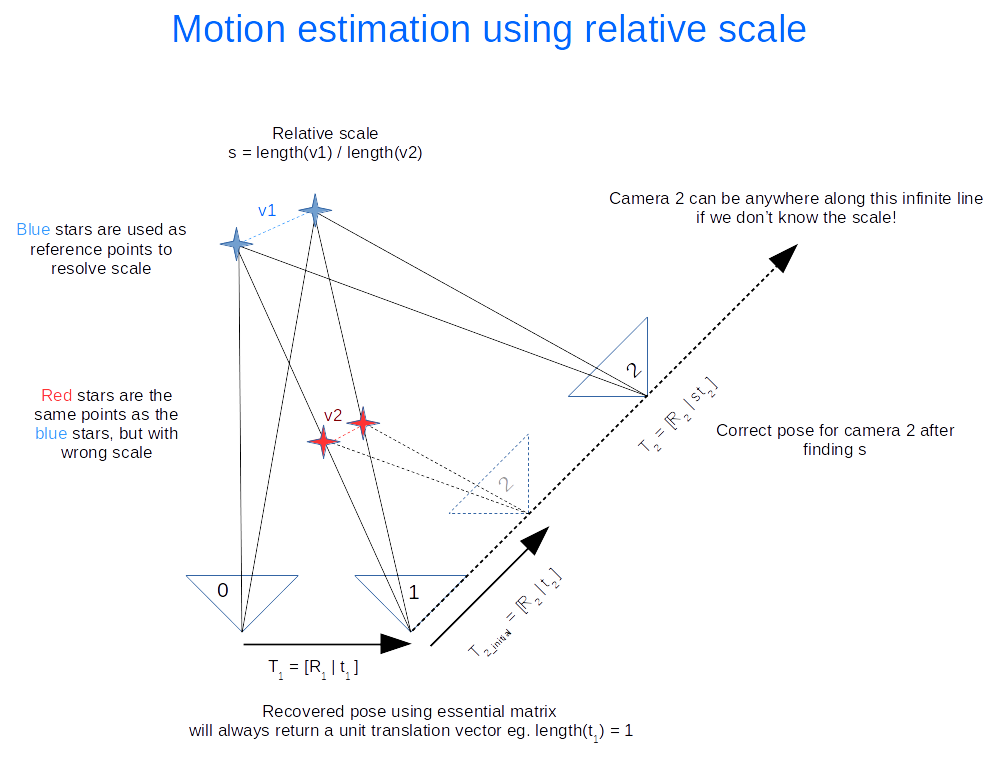
\includegraphics[width=\textwidth]{src/img/nghiaho_2017_sfm_scaling}
    \caption{~\cite{nghiaho_2017}}
    \label{fig:sfm-scaling}
\end{figure}

\section{Export}\ohead{Sebastian Schmitt}
Die rekonstruierten Punkte können exportiert und so in 3D-Animationsprogrammen wie Blender\footnote{https://blender.org} weiterverarbeitet werden.
Dazu wird das Polygon File Format (PLY) verwendet, welches in \autoref{sec:ply-format} genauer erklärt wird.

Die Schnittstelle zum Export ist in der abstrakten Klasse \emph{ModelExporter}, welche in \emph{include/modelexporter.hpp} spezifiziert ist, definiert.
Ziel dieser Lösung ist es mehrere, austauschbare Exporter zu verwenden, wenngleich aktuell nur der PLY Exporter implementiert ist.
Dieser ist in der Klasse \emph{PlyModelExporter} implementiert, welche von \emph{ModelExporter} erbt.
Diese Klasse ist in \emph{include/model-exporters.hpp} spezifiziert und in \emph{src/ply-model-exporter.cpp} implementiert.


\subsection{Polygon File Format}\label{sec:ply-format}
Die Datei beginnt mit einem Header.
In diesem wird der Aufbau der Datei genauer spezifiziert.
Der Header startet dabei immer mit der magischen Zahl \emph{ply}.
In der zweiten Zeile wird mit \emph{format} das verwendete Format sowie die Version des Formats festgelegt.
Verfügbare Formate sind entweder \emph{ascii}, \emph{binary\_little\_endian} sowie \emph{binary\_big\_endian}.
Aktuell gibt es nur Version 1.0.
In dieser Arbeit wird zur Ausgabe das \emph{ascii} Format verwendet.
Auch wenn ein Binärformat gewählt wird, so besteht der Header immer aus ASCII-Zeichen.
Mit dem \emph{element} Keyword beginnt die Beschreibung der verwendeten Elemente sowie deren Anzahl.
Mit \emph{property} können verwendete Eigenschaften der Elemente sowie deren Datentypen festgelegt werden.
In dieser Arbeit werden lediglich \emph{vertex} Elemente verwendet.
Diese haben die Attribute \emph{x}, \emph{y} und \emph{z} sowie \emph{red}, \emph{green} und \emph{blue}.
Eine Beispieldefinition ist in \autoref{lst:ply_vertex_element} zu sehen.
Der Header wird mit dem Keyword \emph{end\_header} beendet.
Darauf folgen alle Elemente in der im Header festgelegten Reihenfolge.
Es ist also nicht nötig zusätzlich den Typ des Elements anzugeben.
Um Beispielsweise einen roten Punkt mit den Koordinaten $\left(1, 2, 3\right)$ zu definieren, braucht man folgenden Eintrag:\\
\emph{1.0	2.0	3.0	255	0	0}

\begin{lstlisting}[numbers=left, breaklines=true, breakatwhitespace=false, label=lst:ply_vertex_element, caption=Beispiel PLY Header für 10 Vertex Elemente mit den Attributen Position und Farbe]
element vertex 10
property float x
property float y
property float z
property uchar red
property uchar green
property uchar blue
end_header
\end{lstlisting}

\subsection{Farben}
Zur Bestimmung der Farben der Punkte gibt es die Klasse \emph{ColorPicker} welche in \emph{include/colors.hpp} spezifiziert und in \emph{src/colors.cpp} implementiert ist.
Diese stelle eine öffentliche, statische Methode bereit welche als Parameter zwei Bilder, zwei Punkte sowie einen Radius annimmt.
Zunächst wird pro Bild über den Radius um den übergebenen Punkt herum die Durchschnittsfarbe bestimmt, danach wird der Durchschnitt beider Farben gebildet.

Leider kann Blender nicht von sich aus Farben in Punktwolken visualisieren.
Möchte man in Blender auch die Farben darstellen, so bietet sich das Addon \emph{Point Cloud Visualizer}\footnote{https://blenderartists.org/t/point-cloud-visualizer/684180} an.
Zur Installation muss lediglich die Datei \emph{space\_view3d\_point\_cloud\_visualizer.py} in den Blender Add-on Einstellungen installiert werden.
Zur Verwendung kann man der 3D View mittels \emph{Add}  $\,\to\,$ \emph{Mesh} $\,\to\,$ \emph{Plane} ein Plane hinzufügen.
Durch drücken der Taste \emph{n} öffnet sich rechts ein Optionsmenü.
Dieses hat als zusätzlichen Punkt nun \emph{Point Cloud Visualizer}.
Hier kann die PLY Datei geladen und gerendert werden\cite{blender_point_cloud_visualizer}.